\documentclass{article}
\usepackage[utf8]{inputenc}
\usepackage{indentfirst}
\usepackage{pdfpages}
\usepackage{float}
\usepackage[
backend=biber,
style=alphabetic,
sorting=ynt
]{biblatex}

\addbibresource{bibliography.bib}

\setlength{\parskip}{0.4em}

\title{Peer-to-Peer Systems and Security \\
        \large{IN2194, SoSe 17} \\
        \huge{Onion Forwarding module} \\
        \small{for Anonymous and Unobservable VoIP Application} \\
        \bigbreak
        \large{\textbf{Interim Report}}}
\author{Team \#27 \\
\textbf{Eiler Poulsen} (03692108), Informatics (M.Sc.) \\
\textbf{Illia Ovchynnikov} (03692268), Informatics (M.Sc.)}
\date{May 2017}

\begin{document}

\maketitle

\section{Application Architecture}
We are looking into creating a multi-threaded architecture, in which incoming requests are intercepted by a single thread (the Selector), queued, and subsequently processed asynchronously by threads (Thread Handlers) from a thread pool. To achieved this goal, we take advantage of the Netty framework\cite{netty}.

One of its main benefits is the concept of pipelines for events; in which a task can be sequentially processed in multiple steps. This is a powerful concept considering the application in question and the data being transported; layered packaged data that must be and processed in multiple steps. Netty also provides us with length prefix framing which is important from a security point of view. The end result is a more secure, non-blocking, high performant, and scalable solution by design.

\begin{figure}[H]
\centering
     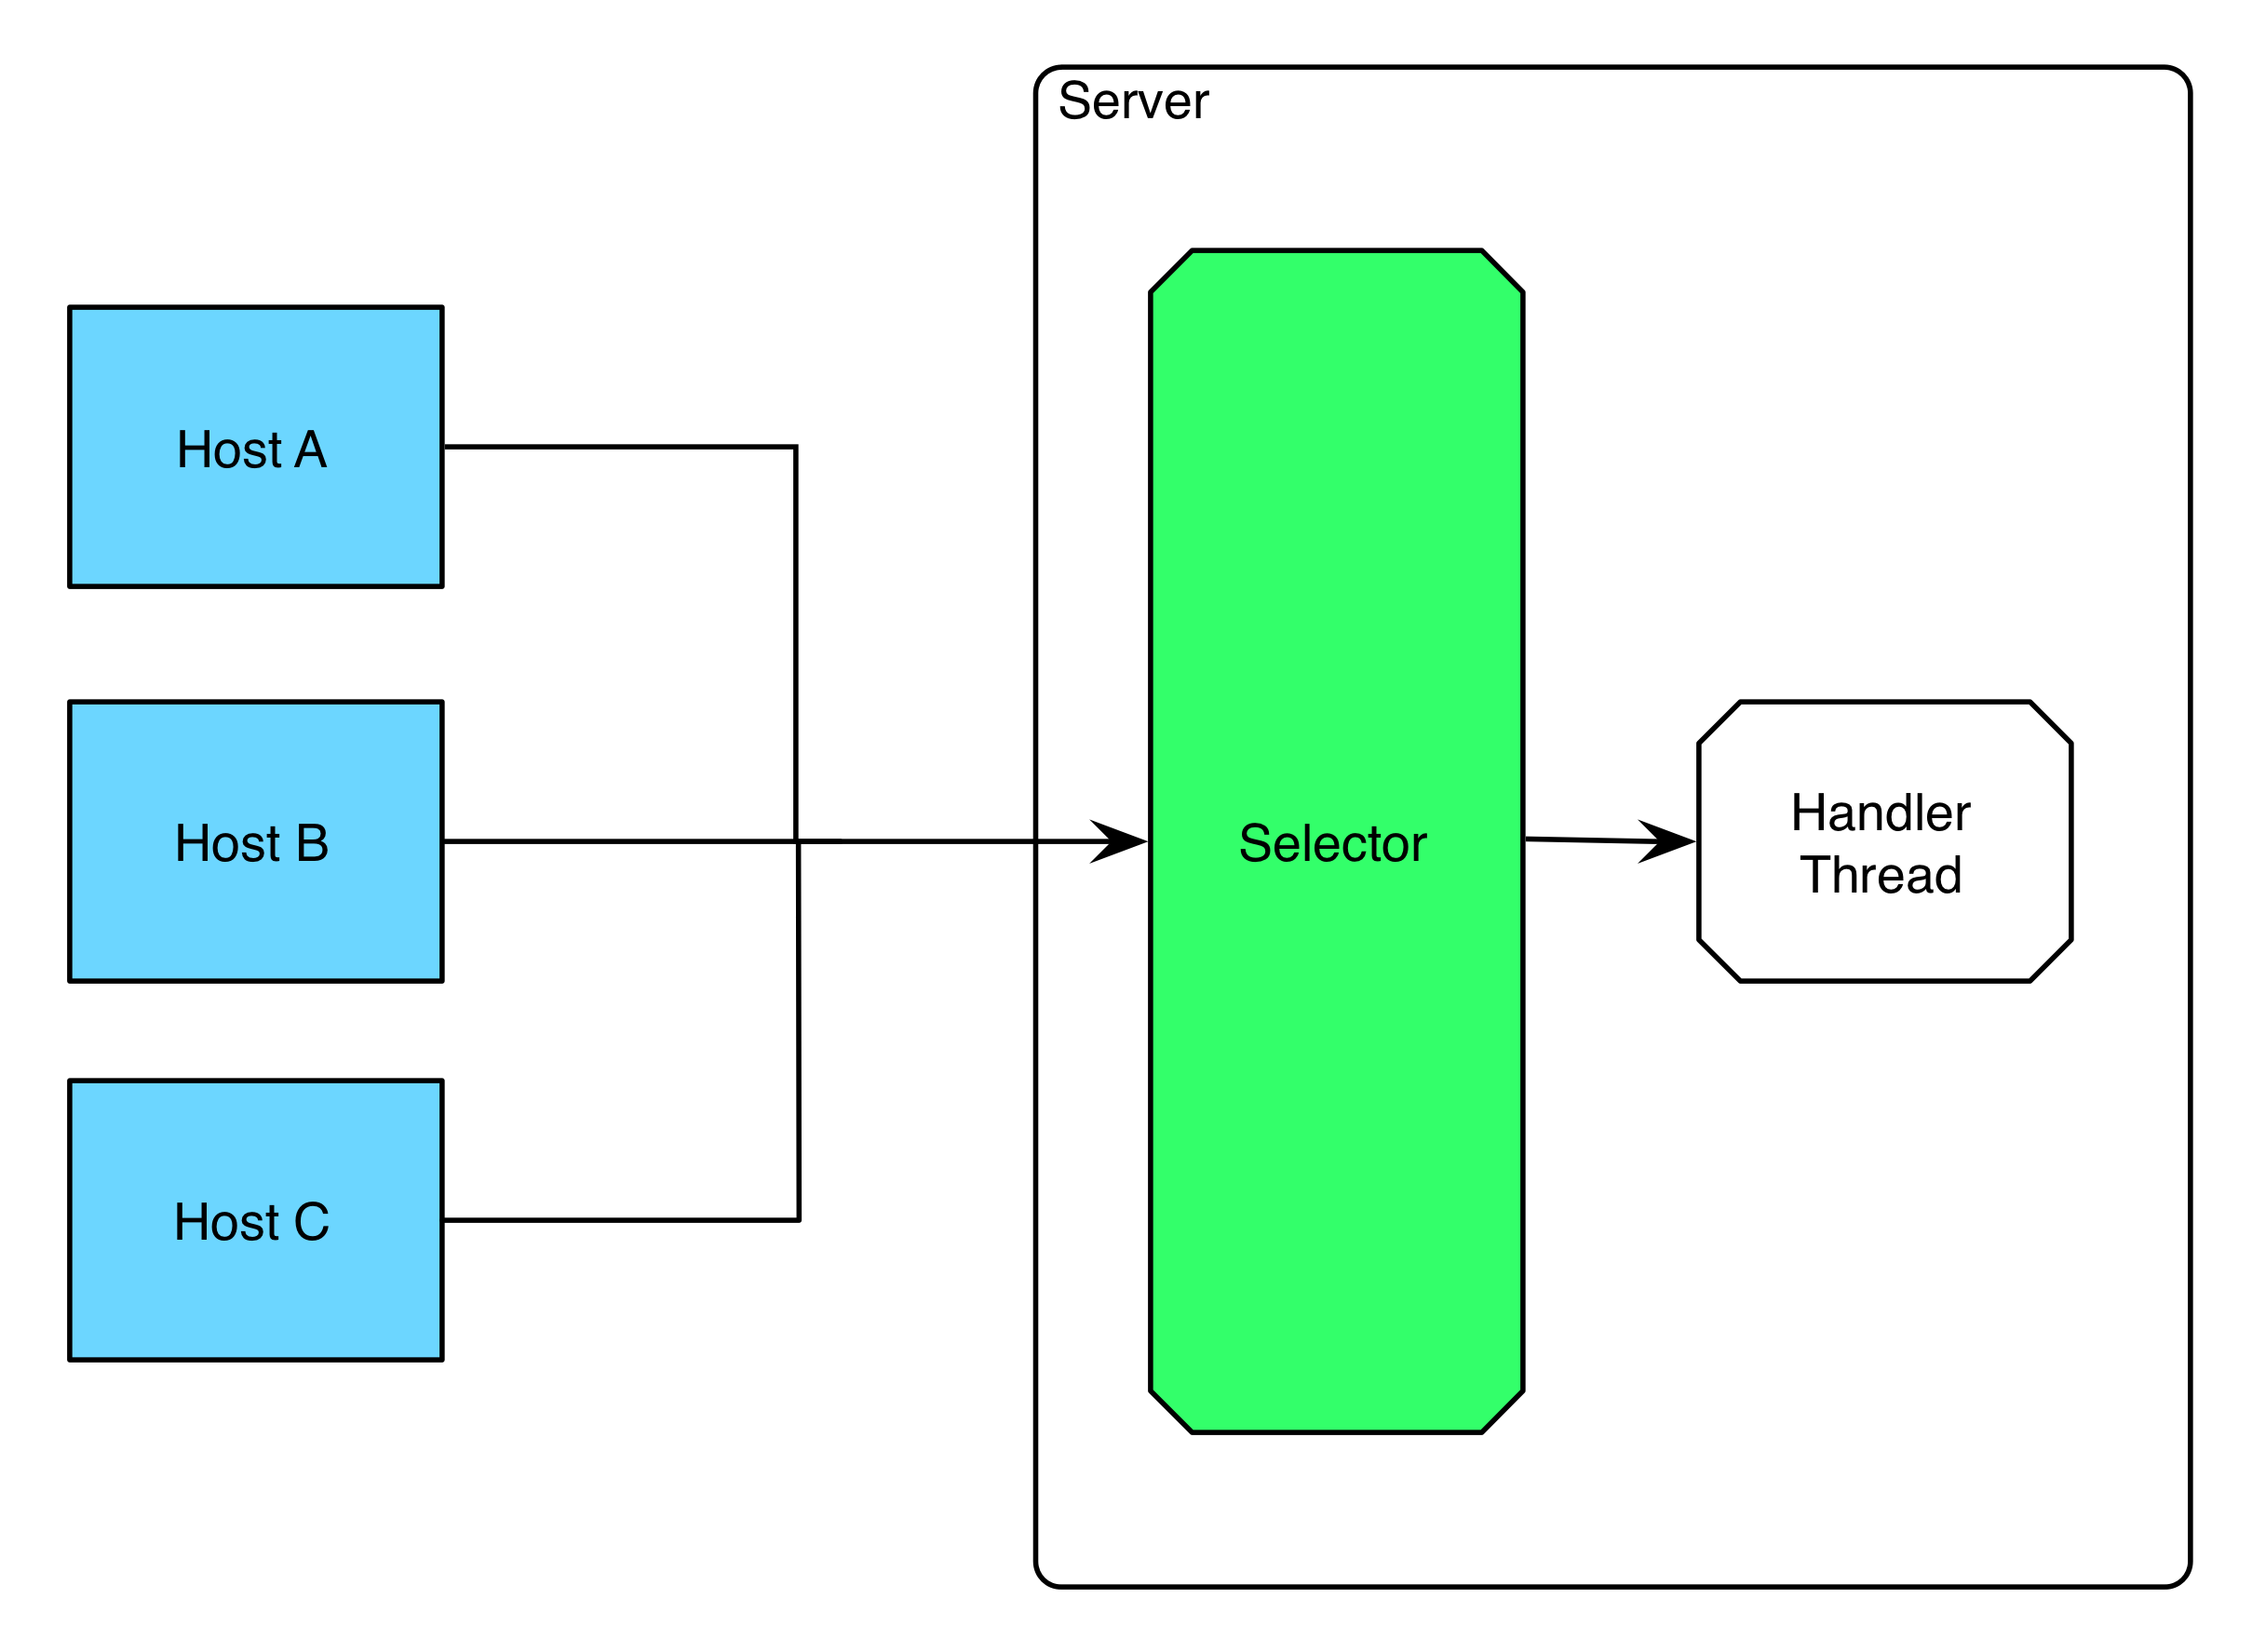
\includegraphics[width=0.75\textwidth]{arc_img1.png}
      \caption{Illustration of Netty's NIO architecture. Credit goes to \cite{netty}.}
\end{figure}

The network library process architecture is as follows, in which the handlers illustrate the sequence of a possible pipeline.

\begin{figure}[H]
\centering
     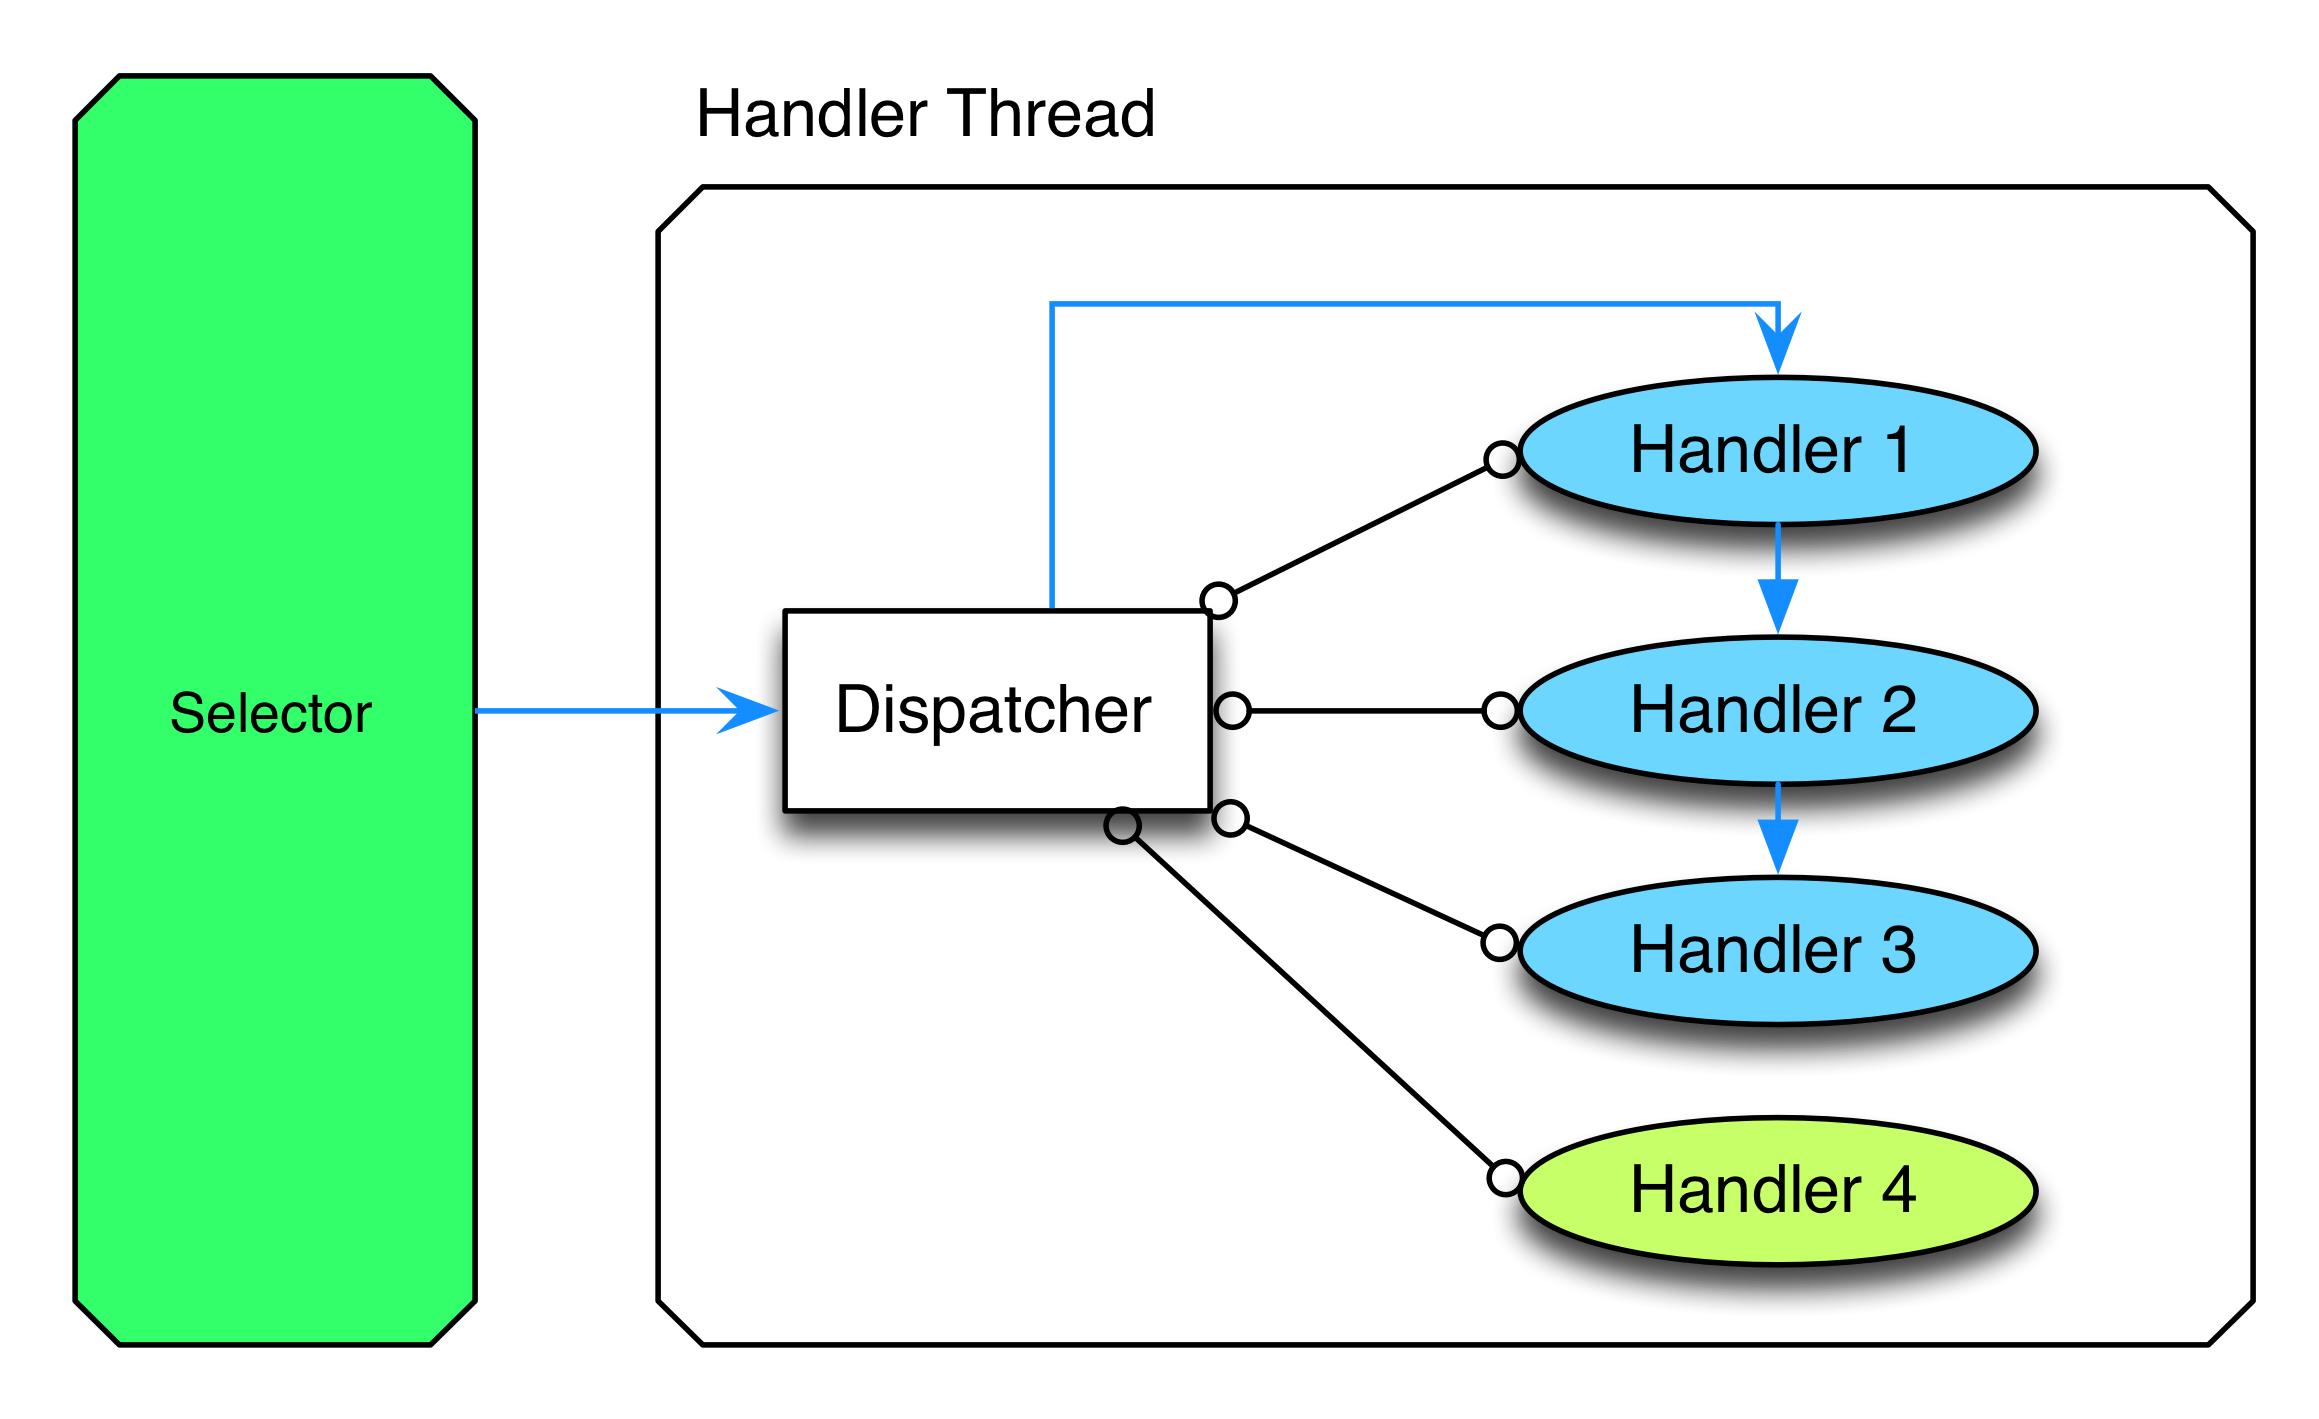
\includegraphics[width=0.75\textwidth]{arc_img2.png}
      \caption{Illustration of the relationship between dispatch service and event handlers. Credit goes to \cite{netty}.}
\end{figure}

%- mention that netty handle length prefix framing for us (google LengthFieldBasedFrameDecoder and LengthFieldPrepender javadocs for details)

\section{Onion Routing}

An origin onion \textit{O} constructs tunnels incrementally, negotiating a symmetric key with each peer on the tunnel, one hop at a time. To begin creating a new tunnel, the \textit{O} sends a TUNNEL CREATE message to the first hop peer \textit{H\textsubscript{1}} in its chosen path. The message's payload contains the first half of the Diffie-Hellman handshake, encrypted to the onion key of \textit{H\textsubscript{1}}.
\begin{figure}[H]
\centering
     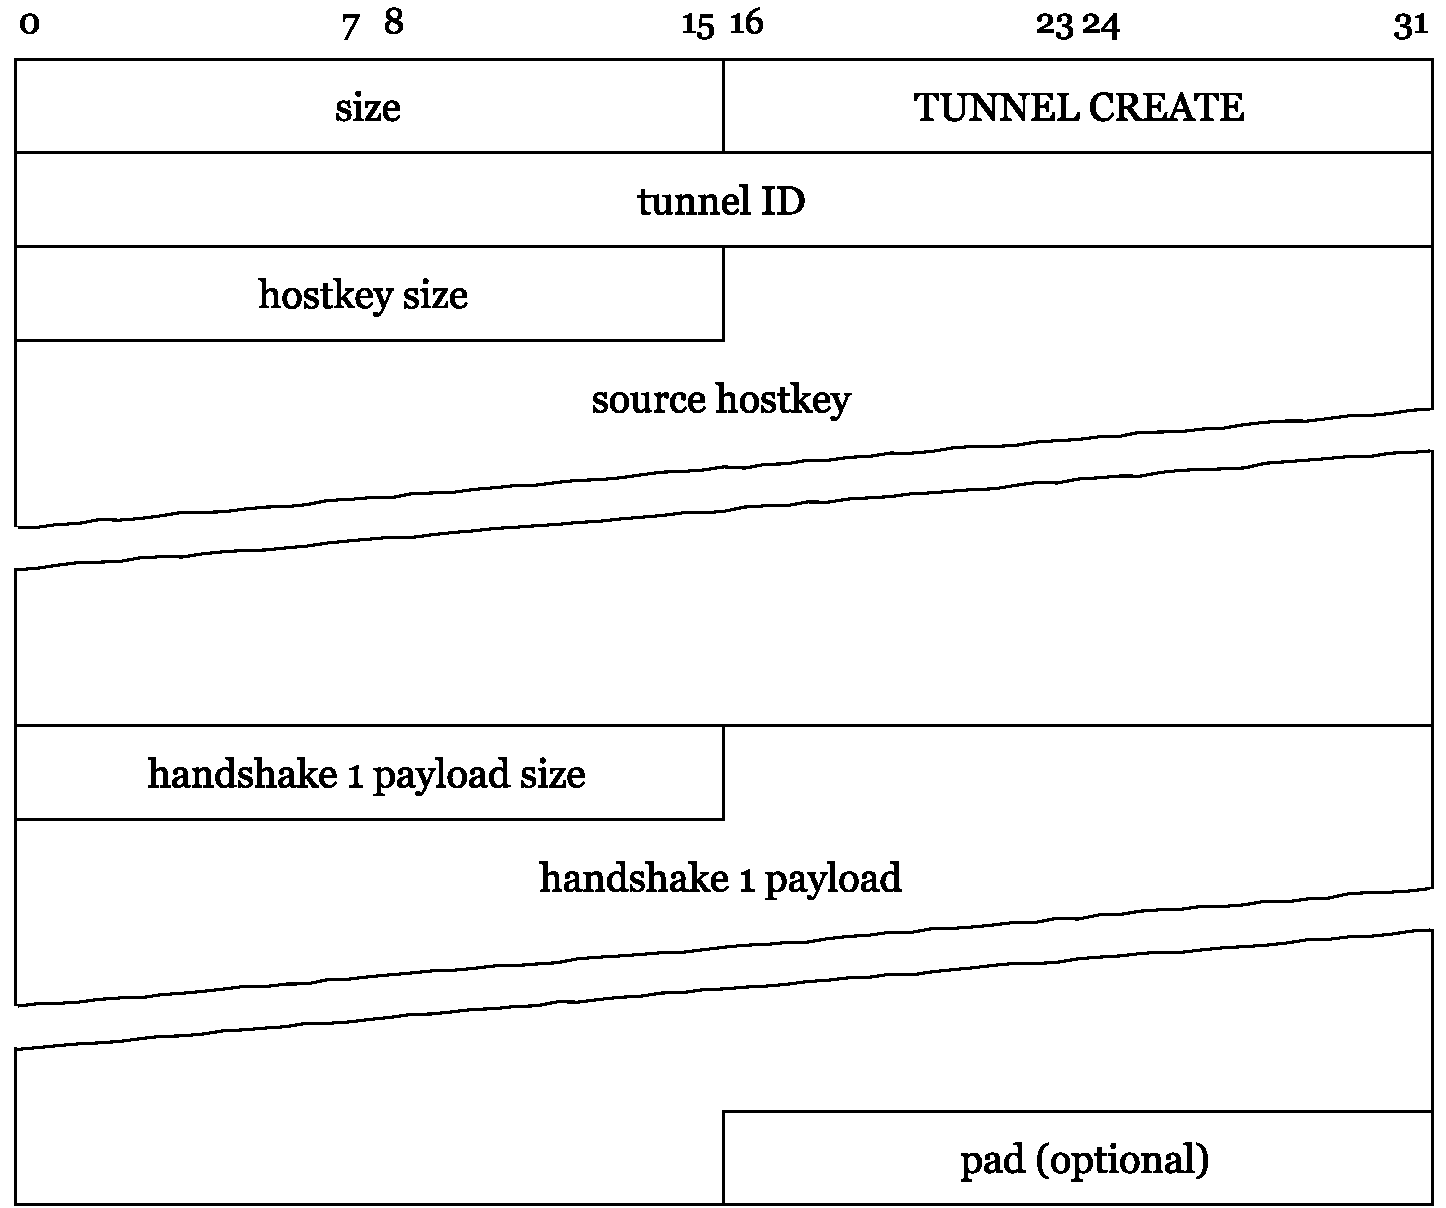
\includegraphics[width=0.8\textwidth]{msg_tunnel_create.pdf}
      \caption{Protocol data unit that represents an intention to perform a handshake}
\end{figure}

\textit{H\textsubscript{1}} then responds with a TUNNEL CREATED message containing the second half of the Diffie-Hellman handshake.

\begin{figure}[H]
\centering
     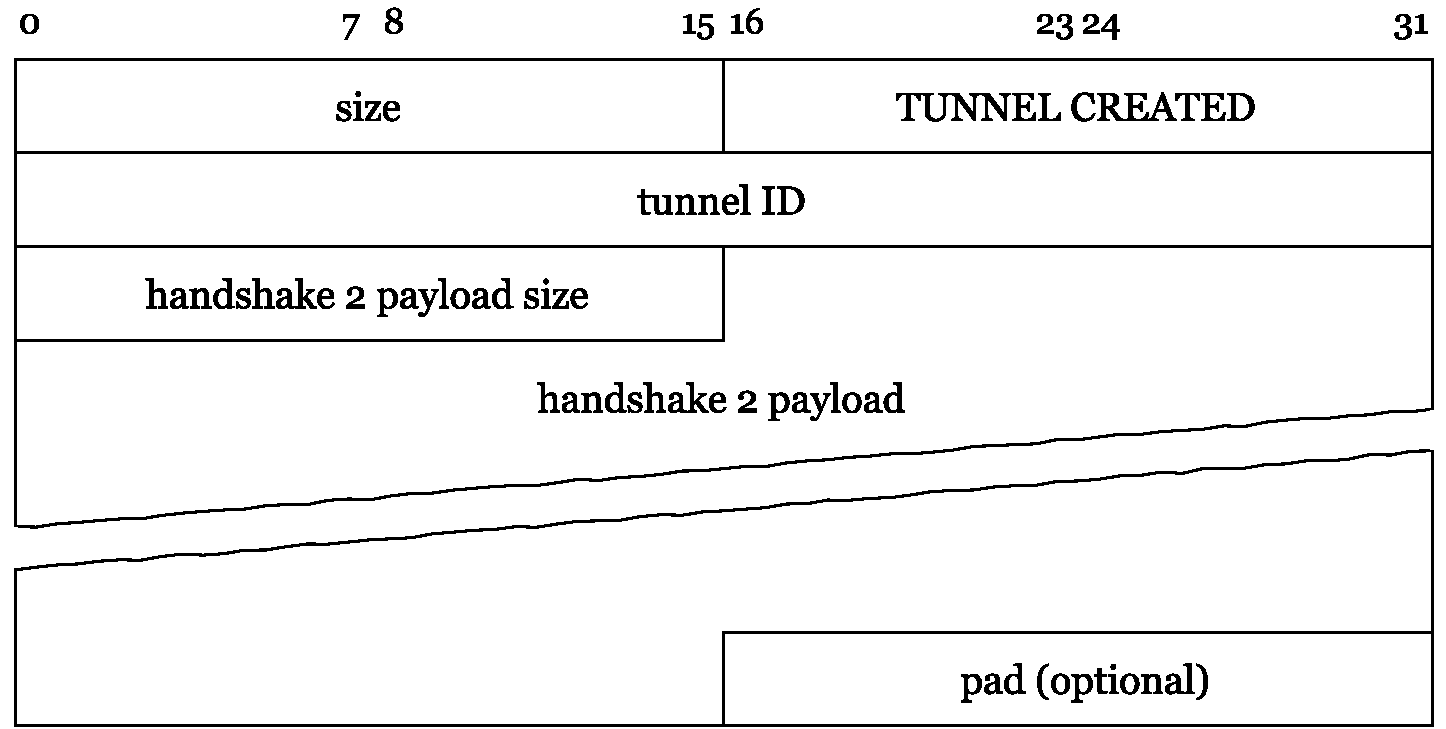
\includegraphics[width=0.75\textwidth]{msg_tunnel_created.pdf}
      \caption{Protocol data unit used to finalize the handshake}
\end{figure}

Once the tunnel has been established, \textit{O} and \textit{H\textsubscript{1}} can communicate securely with the negotiated key \textit{K\textsubscript{1}}.

To extend the tunnel further, \textit{O} sends a TUNNEL EXTEND to \textit{H\textsubscript{1}}, specifying the address of the next onion \textit{H\textsubscript{2}} along with the first half of the Diffie-Hellman handshake for \textit{H\textsubscript{2}}. \textit{H\textsubscript{1}} copies the half-handshake into a TUNNEL CREATE message, and passes it to \textit{H\textsubscript{2}} to extend the tunnel.

\begin{figure}[H]
\centering
     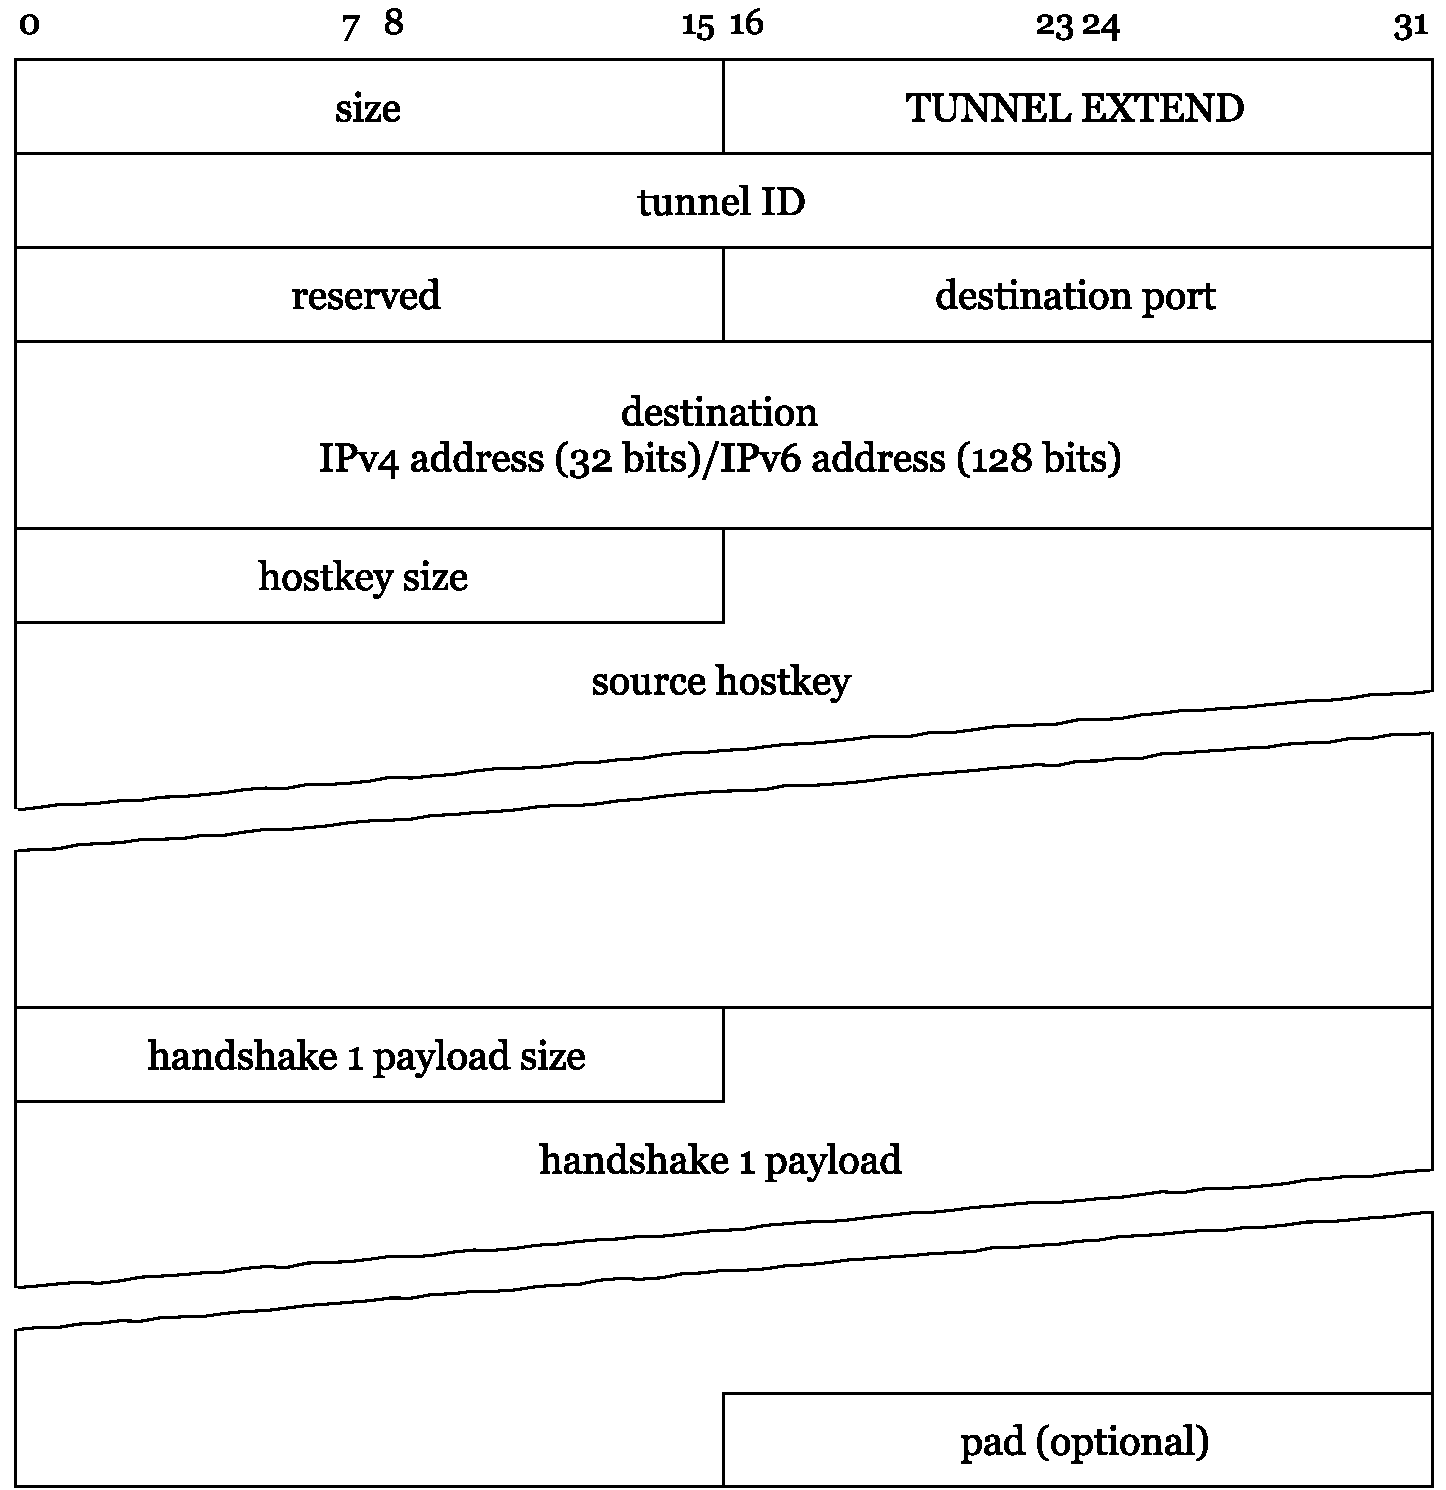
\includegraphics[width=0.75\textwidth]{msg_tunnel_extend.pdf}
      \caption{Protocol data unit that represents an intention to extend the tunnel}
\end{figure}

When \textit{H\textsubscript{2}} responds with a TUNNEL CREATED, \textit{H\textsubscript{1}} wraps the payload into a TUNNEL EXTENDED message and passes it back to \textit{O}. Now the tunnel is extended to \textit{H\textsubscript{2}}, and \textit{O} and \textit{H\textsubscript{2}} share a common session key \textit{K\textsubscript{2}}.
\begin{figure}[H]
\centering
     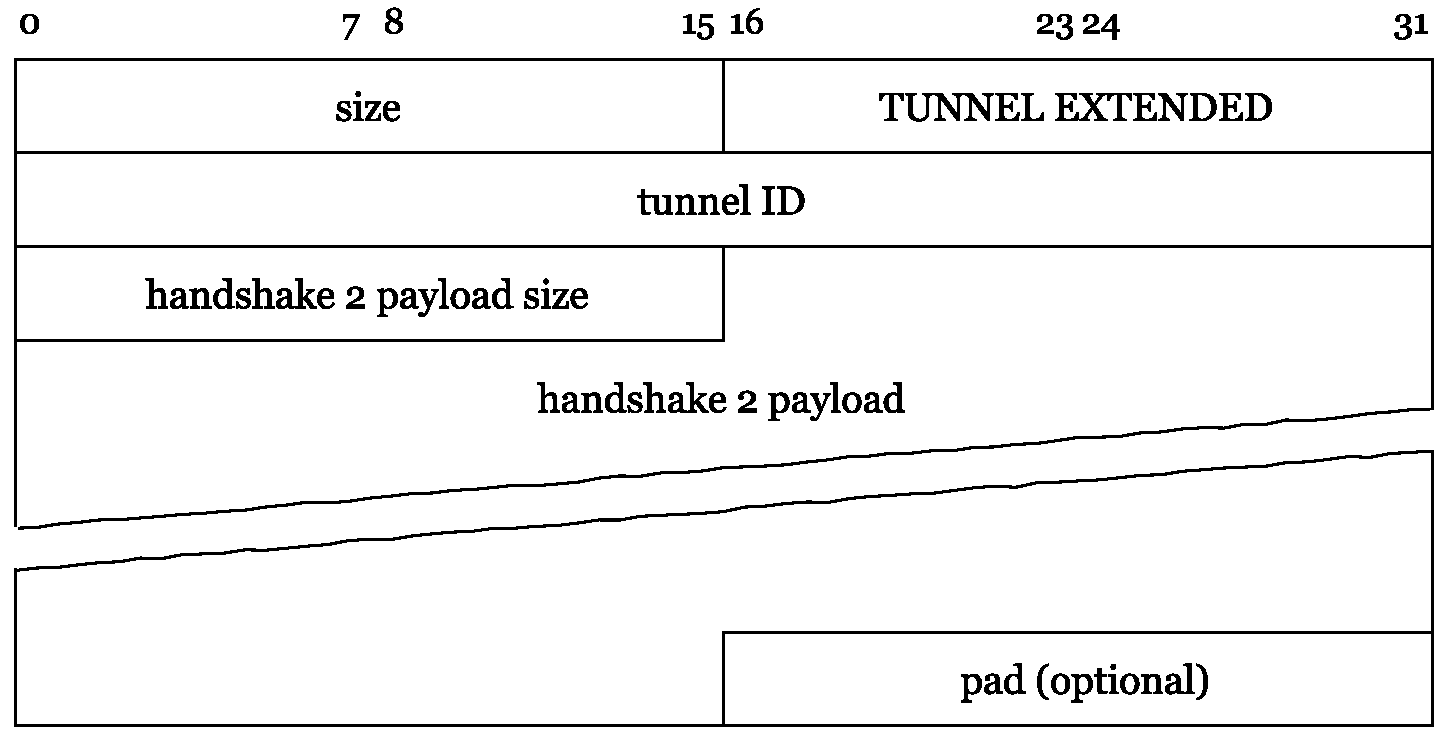
\includegraphics[width=0.75\textwidth]{msg_tunnel_extended.pdf}
      \caption{Protocol data unit used to finalize the handshake during tunnel extension}
\end{figure}

To extend the tunnel to a third node or beyond, \textit{O} proceeds as above, always telling the last node in the tunnel to extend one hop further.

Once \textit{O} has established the tunnel it can relay data in TUNNEL DATA messages. To enable confidentiality, integrity, and authenticity (Authenticated Encryption) message contains message authentication code generated using Encrypt-then-MAC scheme.

\begin{figure}[H]
\centering
     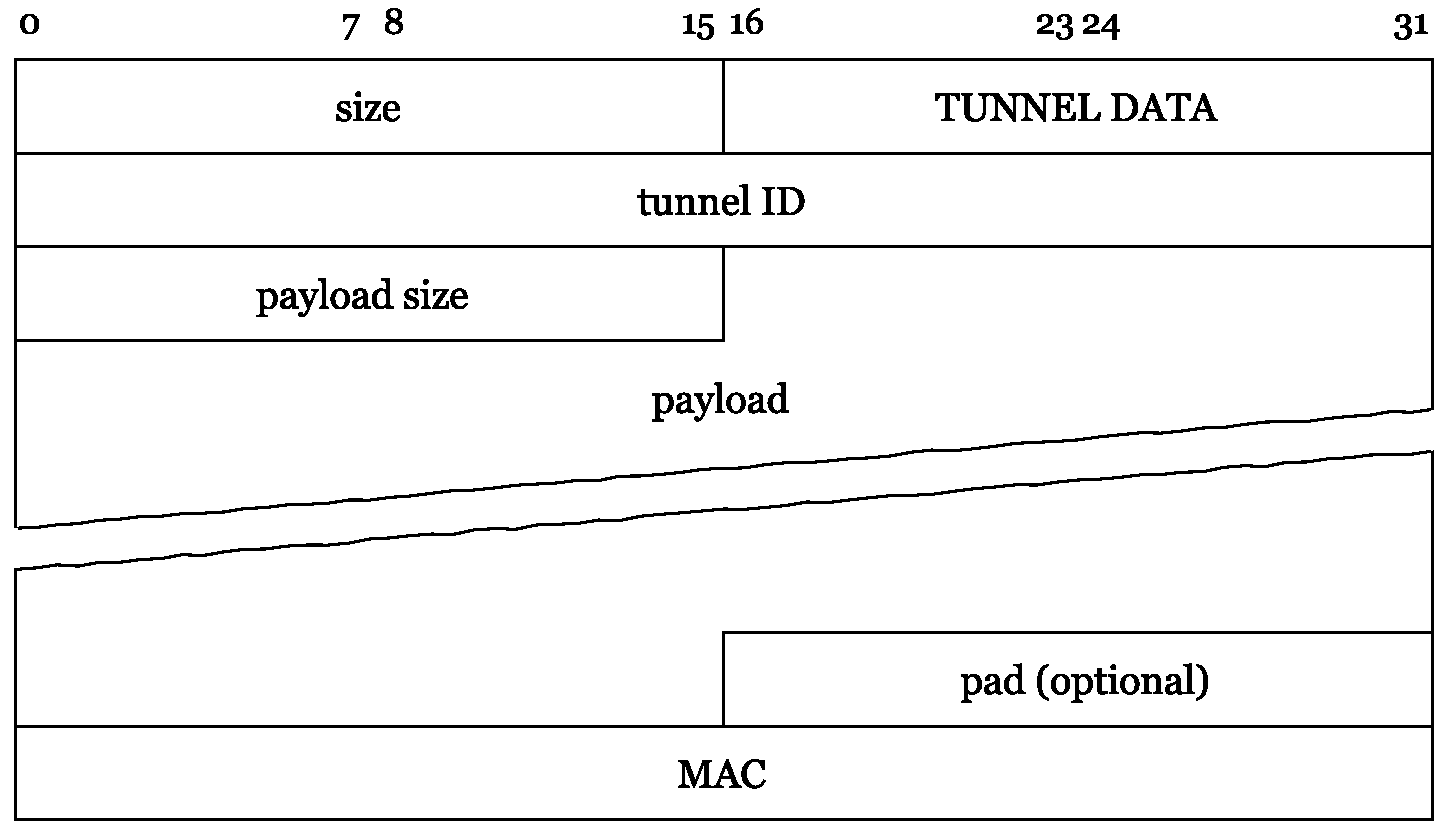
\includegraphics[width=0.75\textwidth]{msg_tunnel_data.pdf}
      \caption{Protocol data unit used to relay data}
\end{figure}

To construct a TUNNEL DATA message addressed to a given \textit{H\textsubscript{n}}, \textit{O} iteratively encrypts the payload with the symmetric key of each hop up to that \textit{H\textsubscript{n}} peer.

Upon receiving a TUNNEL DATA message, an \textit{H\textsubscript{1}} checks whether the message has a valid HMAC, looks up the corresponding tunnel, and decrypts the payload with the session key for that tunnel.  \textit{H\textsubscript{1}} and further peers in the tunnel iteratively unwrap the payload with the session keys shared with each \textit{H\textsubscript{n}} on the tunnel, from the closest to farthest.

To tear down a tunnel, \textit{O} sends a TUNNEL DESTROY message. Each \textit{H\textsubscript{1}} in the tunnel receives the message, tear down all resources associated with this tunnel and passes a new TUNNEL DESTROY message.

\begin{figure}[H]
\centering
     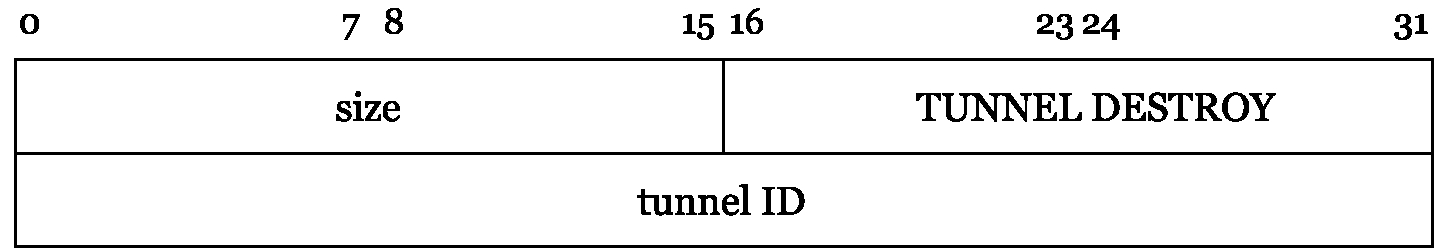
\includegraphics[width=0.75\textwidth]{msg_tunnel_destroy.pdf}
      \caption{Protocol data unit used to notify about tunnel invalidation}
\end{figure}

TUNNEL ERROR message used to indicate different errors that arise during onion communication. It contains specific error code and may contain tunnel identifier and an address of a peer, that caused this error.

\begin{figure}[H]
\centering
     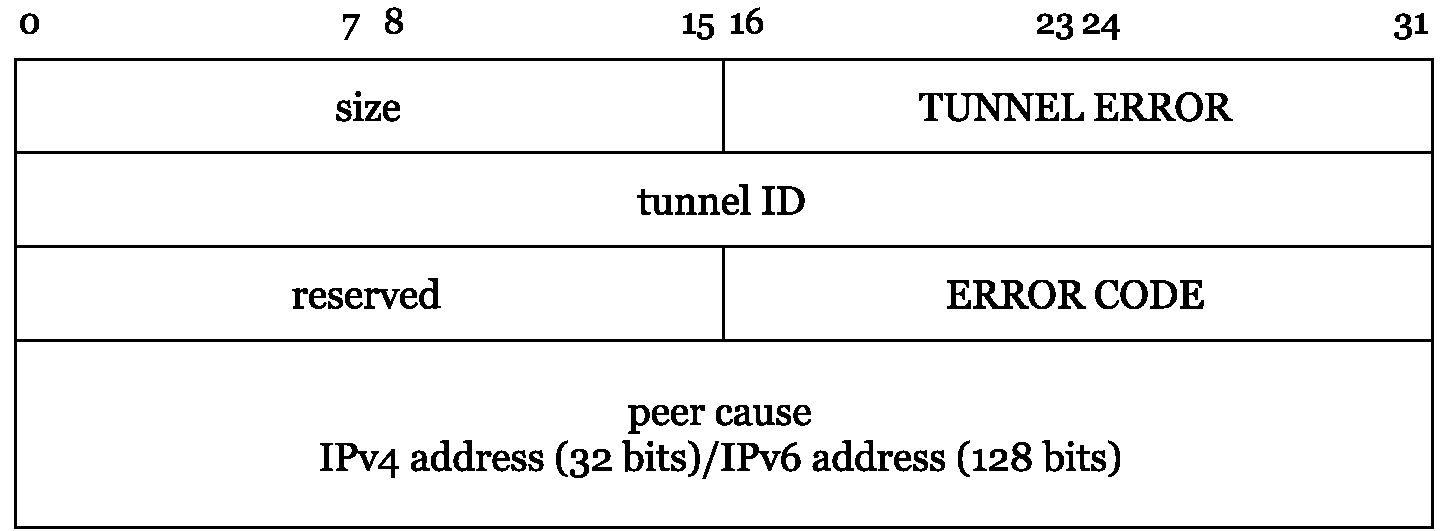
\includegraphics[width=0.75\textwidth]{msg_tunnel_error.pdf}
      \caption{Protocol data unit used to notify onions about communication error of different types}
\end{figure}

It's a responsibility of a peer which founds and error to notify peers about error with appropriate ERROR CODE and peer cause address. Errors are propagated back to the tunnel originator \textit{O} that may decided to tear down a tunnel then.

\medskip

\nocite{torproject}
\nocite{netty}


\printbibliography
\end{document}
